Before presenting the different LSH methods, let's start by presenting the
global approach shared by all of them, it consists of three steps:
\begin{itemize}
    \item Hashing.
    \item Amplification.
    \item Bucketing.
\end{itemize}

\subsection{Hashing}
This step consists of applying a set of hashing functions $H = (h_1, h_2, ..,
    h_m)$ on the $n$ data points to get their \glspl{signature}. It's the step that
makes the difference between the hashing methods as it is what makes the
effect of choose the hash family clearer. At the end of this step, the
result is a matrix where each data points is presented by its signature,
this matrix is called signature matrix.

$$\begin{bmatrix} h_1 (x_1) & h_1 (x_2) & \cdots & h_1 (x_n) \\
        h_2 (x_1) & h_2 (x_2) & \cdots & h_1 (x_n) \\
        \cdots    & \cdots    & \cdots & \cdots    \\
        h_m (x_1) & h_m (x_2) & \cdots & h_m (x_n)\end{bmatrix}$$

This step of bucketing is contributing on reducing the complexity of the search
process by reducing the dimension of the data points and representing them on a
latent space. It lets the search process dealing with a reduced size of vector
rather than to perform on the entire vectors.

\subsection{Amplification}
The amplification step the signature matrix from the previous section is divided
into $b$ bands each one of size $r$. This means that, for a set of hashing
functions ($h_1$, $h_2$, $\cdots$, $h_p$) such that $p = b*r$, we will have this
set divided into $b$ sub-sets ([$h_{1}$, $\cdots$ $h_{r}$], [$h_{r+1}$, $\cdots$
        $h_{2r}$], $\cdots$, [$h_{(b-1)*r + 1}$, $\cdots$ $h_{p = b*r}$]). The figure
\ref{fig:amplification_divide_rb} shows how the signature is divided.

\begin{figure}[h]
    \centering
    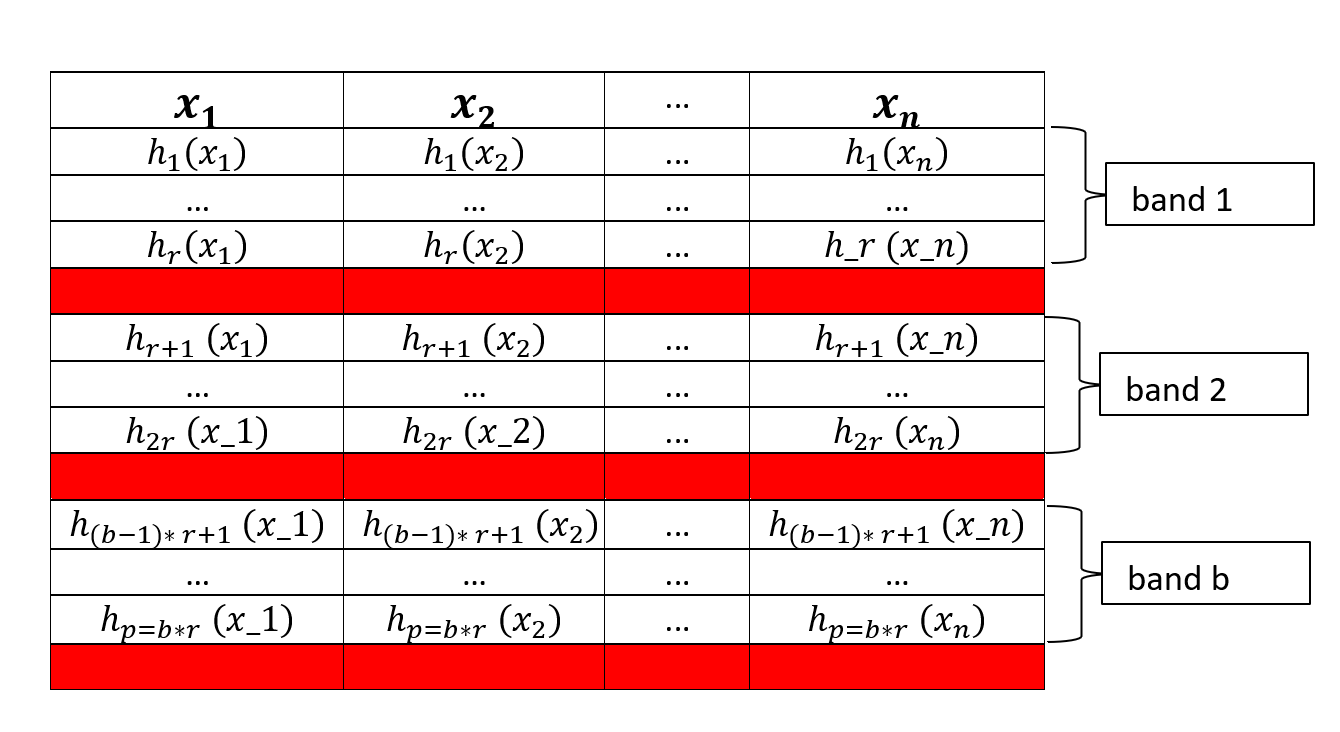
\includegraphics{state_of_the_art/steps/amplification_step.png}
    \caption{Amplification step illustration: Division of the signature matrix}
    \label{fig:amplification_divide_rb}
\end{figure}

The intuition behind doing such dividing, is to minimize the collisions between
points that are not similar. In another way, we aim to minimize the false
positives that may occur when we consider one hash value at a time while making
buckets by not considering one hash value at a time but regrouping them into $b$
set of hashing values.

\subsection{Bucketing}
The bucketing step is the last step in the process in each of the LSH methods.
It consists of creating buckets and assigning data points to them. To do this,
it gets the output of the amplification step which are hashing values divided
into subsets such that each subset of a data point $x$ is used to identify the
bucket in which $x$ is assigned. Each data point can be mapped to different
buckets as it has different subsets of hashing values.

The figure \ref{fig:bucketing_example} show an example on how the different data
points are assigned to buckets.

\begin{figure}[h]
    \centering
    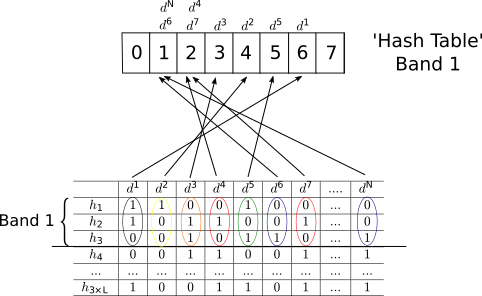
\includegraphics{state_of_the_art/steps/bucketing_step.png}
    \caption{Bucketing step example}
    \label{fig:bucketing_example}
\end{figure}

At the end of this step, the data points sharing the same bucket are considered
as candidates to be similar.

This step of bucketing is contributing on reducing the complexity of the search
process by focusing its search on the subset of data points that share at least
one bucket with the query point rather than having to do the search over all the
data points.
